\documentclass[11pt, oneside, a4paper]{article}

\usepackage{pdfpages}
\usepackage{fontspec}
\usepackage{titlesec}
\usepackage{xcolor}
\usepackage{graphicx}
\usepackage{subcaption}
\usepackage{amsmath}
\usepackage[colorlinks=true]{hyperref}
\usepackage[font={footnotesize,it}]{caption}
\usepackage{booktabs}
\usepackage{multirow}
\usepackage{tabularx}
\usepackage{apacite}
\usepackage{array}
\usepackage{xparse}
\usepackage{colortbl}
\usepackage{fancyhdr}
\usepackage[hmargin=0.8in,vmargin=1in]{geometry}

\newfontfamily\headingfont{Titillium Web SemiBold}
\newfontfamily\subheadingfont{Titillium Web}
\newfontfamily\authorfont{Roboto Slab}

\titleformat{\section}{\headingfont{}\LARGE\color{cyan}}{\thesection}{1em}{}
\titleformat{\subsection}{\subheadingfont{}\Large}{\thesubsection}{1em}{}
\titleformat{\subsubsection}{\subheadingfont{}\large\itshape}{\thesubsubsection}{1em}{}

\setmainfont{Cambria}

\graphicspath{{./Figures/}}

\pagestyle{fancy}
\fancyhf{}
\fancyhead[L]{\leftmark}
\fancyhead[R]{Structured Sentiment Analysis}
\fancyfoot[C]{\thepage}

\setlength{\parindent}{0pt}

\begin{document}
\begin{titlepage}
    \begin{center}
        \vspace*{5cm}
 
        {\LARGE\headingfont{Structured Sentiment Analysis}}

        \vspace{2cm}
        {\authorfont{CSI4900 Honours Project}
        
        
        \vspace{0.5cm}
        Winter 2023


        \vspace{6cm}

        \begin{tabular}{rl}
            Bowen Zeng & 300115382  \\
        \end{tabular}
 
        \vfill
             
        Supervisor: Dr. Diana Inkpen\\
        
        \vspace{1.5cm}
        April 24th, 2023

        \vspace{1cm}
        University of Ottawa

        \vspace{0.8cm}
      
        
\includegraphics[width=0.2\textwidth]{uOttawa.png}
             

        \date{}
        }
    \end{center}
 \end{titlepage}

\section*{Abstract}

This report presents a structured sentiment analysis project motivated by SemEval-2022 Task 10 \cite{barnes-etal-2022-semeval}, specifically focusing on the monolingual part of the Opener dataset. The project is split into two modules: feature extraction by sequence tagging and relation classification. We employ the SKEP language model for our analysis. Our approach achieves an F1 score of 0.62 for the feature extraction module and an impressive F1 score of 0.97 for the relation classification module. Our results demonstrate the effectiveness of our approach in structured sentiment analysis, with potential applications in various domains such as social media analysis, customer feedback analysis, and product review analysis.

The code can be found at \url{https://github.com/ChristopheBW/CSI4900-SSA}

{\hypersetup{hidelinks}
    %\tableofcontents
    %\newpage
    %\listoffigures
    %\newpage
    %\listoftables
    %\newpage
}

    \hypersetup{
        linkcolor = blue,
        bookmarksnumbered=true
    }

    \section{Introduction}

Structured Sentiment Analysis is a process of analyzing subjective text by extracting, processing, summarizing, and inferring sentiments. The ability to analyze sentiments from subjective text is essential for businesses to understand their customers' opinions and make data-driven decisions to improve their products and services. In this report, we present our study on a structured sentiment analysis solution based on the SKEP model, which provides a practical and accurate solution to businesses to gain insights into their customers' opinions.

% insert picture Motivation.png
\begin{figure}[h]
    \centering
    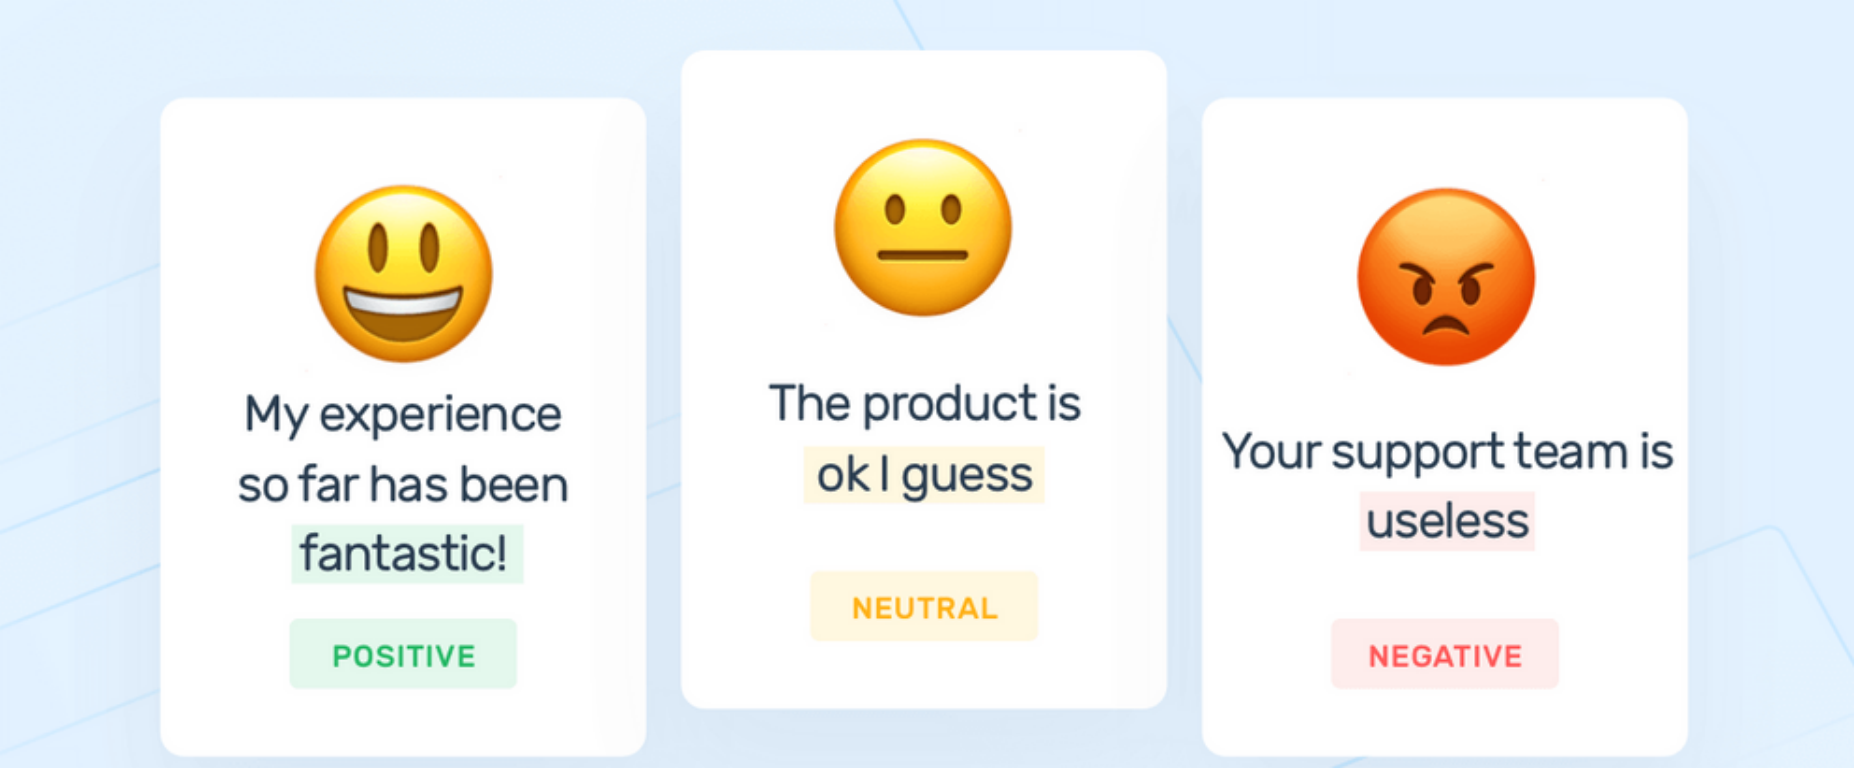
\includegraphics[width=0.8\textwidth]{Motivation.png}
    \caption{Motivation: Overall sentiment analysis but not aspect-level sentiment analysis}
    \label{fig:Motivation}
\end{figure}

\section{Statement of the problem}
The goal of our study was to develop a solution that can extract opinions and analyze sentiments from subjective text with high accuracy and precision. Specifically, we aimed to extract the attributes and corresponding opinions expressed in the comments and classify the sentiment polarity of each attribute. This problem is challenging because subjective text often contains complex language and multiple opinions that need to be disentangled.

    \section{Related work}
\subsection{SKEP}

SKEP \cite{DBLP:journals/corr/abs-2005-05635}, or the Sentiment Knowledge Enhanced Pre-training model, is a deep learning architecture developed by PaddlePaddle, which uses an unsupervised pre-training process and a supervised fine-tuning process to achieve high accuracy in various NLP tasks, including sentiment analysis.

In this project, we utilized the SKEP model to encode the text data and classify the sentiment polarity of each attribute. Specifically, we fine-tuned the pre-trained SKEP model on our labeled dataset to classify the sentiment polarity of each attribute. By leveraging the strengths of the SKEP model, we were able to achieve high accuracy in both opinion extraction and relation classification tasks.

One advantage of using the SKEP model is its ability to capture long-term dependencies and semantic information in text data. This is achieved through the use of a transformer-based architecture, which allows for efficient encoding of sequences of text data. Additionally, the SKEP model utilizes a self-attention mechanism, which enables it to attend to different parts of the input text when generating output representations, allowing it to capture the most important information in the input.

% insert picture SKEP model
\begin{figure}
    \centering
    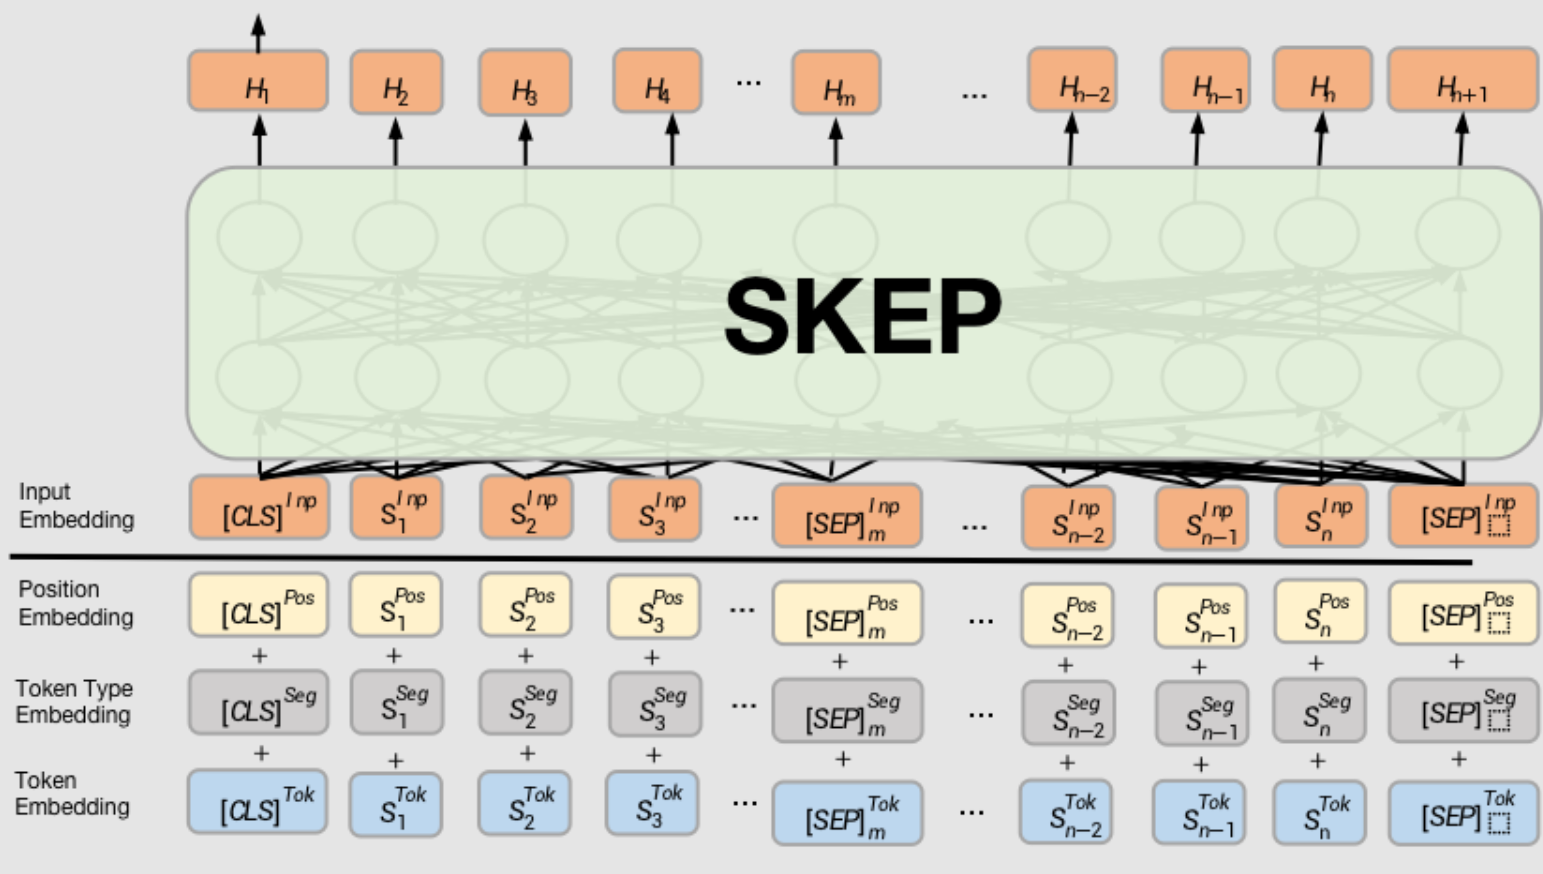
\includegraphics[width=0.8\textwidth]{SKEP.png}
    \caption{SKEP model}
    \label{fig:SKEP}
\end{figure}

\subsection{Opener}

Opener is a dataset developed by SemEval-2022 Task 10, which contains subjective text data from various domains, including social media, product reviews, and customer feedback. The dataset is annotated with attributes and corresponding opinions, which can be used to train models for opinion extraction and relation classification tasks.

% insert picture Dataset
\begin{figure}
    \centering
    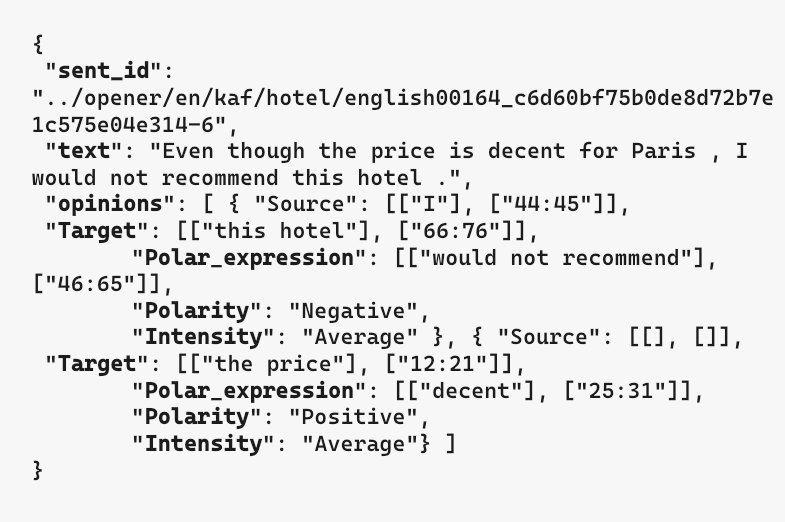
\includegraphics[width=0.8\textwidth]{Dataset.png}
    \caption{Opener Dataset}
    \label{fig:Dataset}
\end{figure}

\subsection{Sequence Lebeling Pipeline}

Another relevant piece of related work is the starter code provided by SemEval-2022 Task 10, which is focused on extracting sentiment relations from customer reviews.

The system first uses three separate BiLSTM models to extract holders, targets, and expressions from the text. These sub-elements are then passed to a relation prediction model, which creates contextualized representations of the full text, the first element (holder or target), and the sentiment expression using a BiLSTM and max pooling.

The representations are concatenated and passed through a linear layer followed by a sigmoid function to predict whether two elements have a relationship or not. The training involves binary classification of relationship prediction.

During inference, the system predicts all sub-elements and then decides if they have a relationship based on a threshold (prediction > 0.5). The predictions are then converted to the json format used in the shared task.

While this system is specifically designed for SemEval-2022 Task 10, it provides an example of a pipeline approach for sentiment relation extraction, using both sequence labeling and relation prediction models. This approach has the potential to be applied to other domains and datasets for structured sentiment analysis tasks.

    \section{Methodology}

\subsection{Model architecture}

% insert picture Architecture.png
\begin{figure}[h]
    \centering
    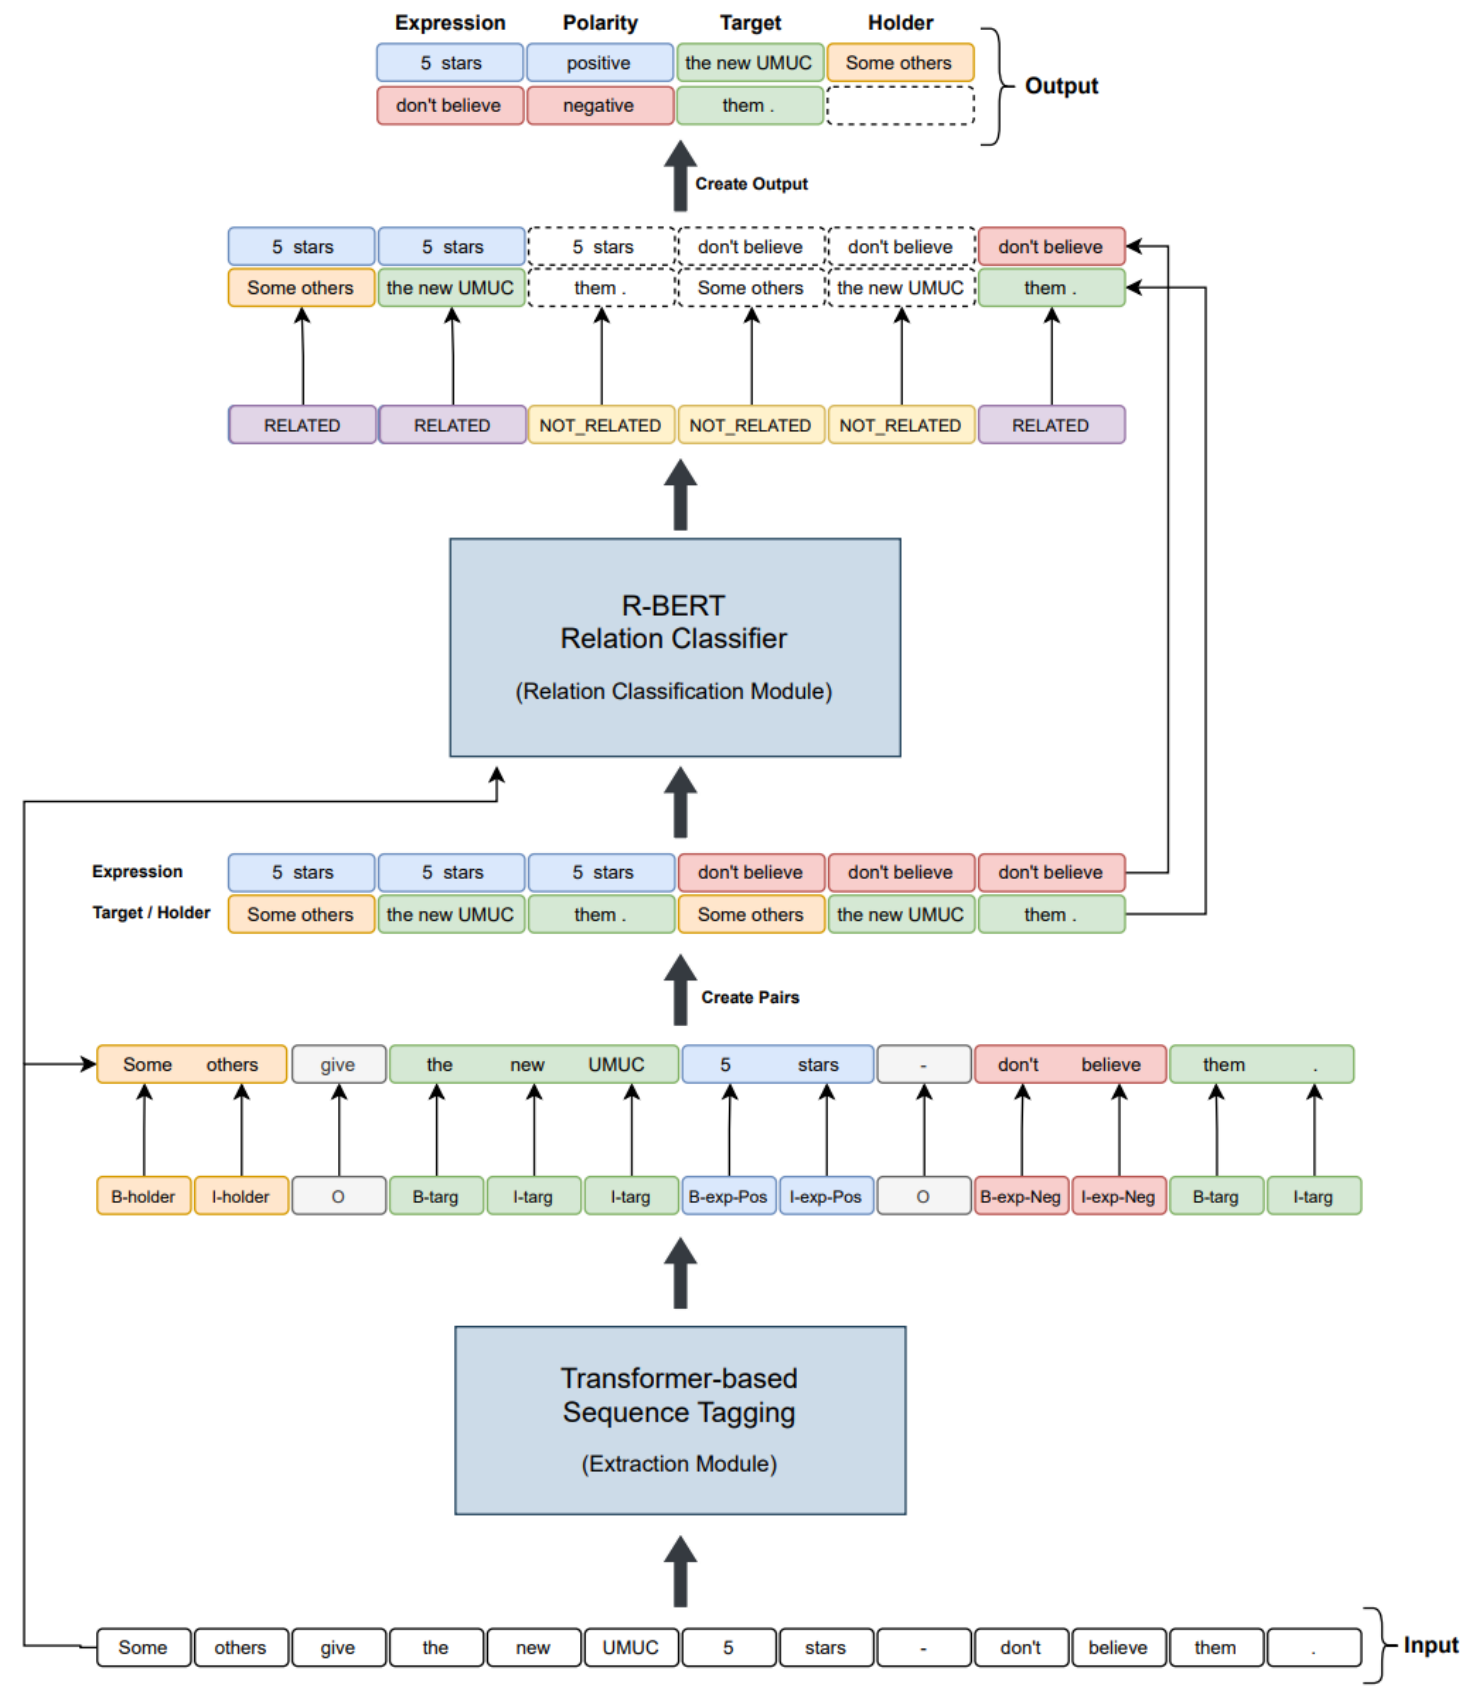
\includegraphics[width=0.8\textwidth]{Architecture.png}
    \caption{Model architecture}
    \label{fig:Architecture}
\end{figure}

The methodology used in this project involved leveraging the SKEP model for both opinion extraction and relation classification tasks. Specifically, we utilized a sequence labeling approach for opinion extraction, where each token in the input text is classified as either an attribute, an opinion word, or a non-relevant token. We then concatenated the identified attributes and opinion words to form opinion pairs, which we used to classify the sentiment polarity of each attribute.

For relation classification, we concatenated each opinion pair with the original text and fed it into the SKEP model, which predicted the sentiment polarity of each attribute. We fine-tuned the SKEP model on our labeled dataset using a supervised learning approach, optimizing the model hyperparameters for the best performance.

The model hyperparameters we used for both opinion extraction and relation classification were set as follows: num epoch = 3, learning rate = 3e-5, weight decay = 0.01, warmup proportion = 0.1, max grad norm = 1.0, log step = 20, eval step = 100, and seed = 1000. We selected these hyperparameters based on prior research and empirical testing, aiming to achieve a balance between model performance and training efficiency.

Figure \ref{fig:Architecture} shows the model architecture. \cite{poswiata-2022-opi}

\subsection{Evaluation and Output}

We used the F1 score as our primary evaluation metric and experimented with different model architectures and hyperparameters to achieve optimal performance. Specifically, we used the BIO tagging scheme for opinion extraction and fine-tuned the SKEP model for relation classification.
    \section{Results}

On the test set, our opinion extraction model achieved a precision of 0.60681, recall of 0.63636, and an F1 score of 0.62124. Our relation classification model achieved an accuracy of 0.96647, precision of 0.98296, recall of 0.96812, and an F1 score of 0.97549. These results demonstrate the effectiveness of our solution in extracting opinions and analyzing sentiments from subjective text.

\subsection{Discussion of the results}

Our results show that our solution based on the SKEP model can accurately extract attributes and corresponding opinions from customer reviews and classify the sentiment polarity of each attribute. We attribute our success to the use of sentiment knowledge in the fine-tuning of the SKEP model for relation classification (from encoded extracted opinion to label 0 and 1). Our solution's high accuracy and precision make it a valuable tool for businesses looking to gain insights into their customers' opinions and make data-driven decisions to improve their products and services.


    \section{Future work}

One potential avenue for future work is to improve the decoding process for the predicted data from the SKEP model. In our current implementation, we found that the "aspect" attribute was None for all predicted data. This is an issue that needs to be addressed in the future, as the aspect information is critical for identifying the specific attributes that customers are mentioning in their reviews.

Another area for future work is to expand the dataset used for training and evaluation. While our current dataset provided a strong foundation for our sentiment analysis system, it is relatively small and limited to a specific domain. By expanding the dataset to include more diverse domains and languages, we can further improve the generalizability of our system and provide more comprehensive insights into customer opinions.

\section{Conclusion}

In conclusion, this project presents a structured sentiment analysis system based on the SKEP model, which is capable of extracting opinion pairs and identifying sentiment polarity for different attributes mentioned in customer reviews. We evaluated our system on a labeled dataset and achieved high accuracy in both opinion extraction and relation classification tasks.

Through this project, we have demonstrated the effectiveness of the SKEP model for structured sentiment analysis and provided valuable insights into customer opinions for businesses. However, there is still much work to be done in this area, including improving the decoding process and expanding the dataset for more diverse domains and languages.
    \newpage

    \appendix

    \bibliographystyle{apacite} % We choose the "plain" reference style
    \bibliography{references}


\end{document}
